% Created by tikzDevice version 0.12.6 on 2024-04-16 16:18:12
% !TEX encoding = UTF-8 Unicode
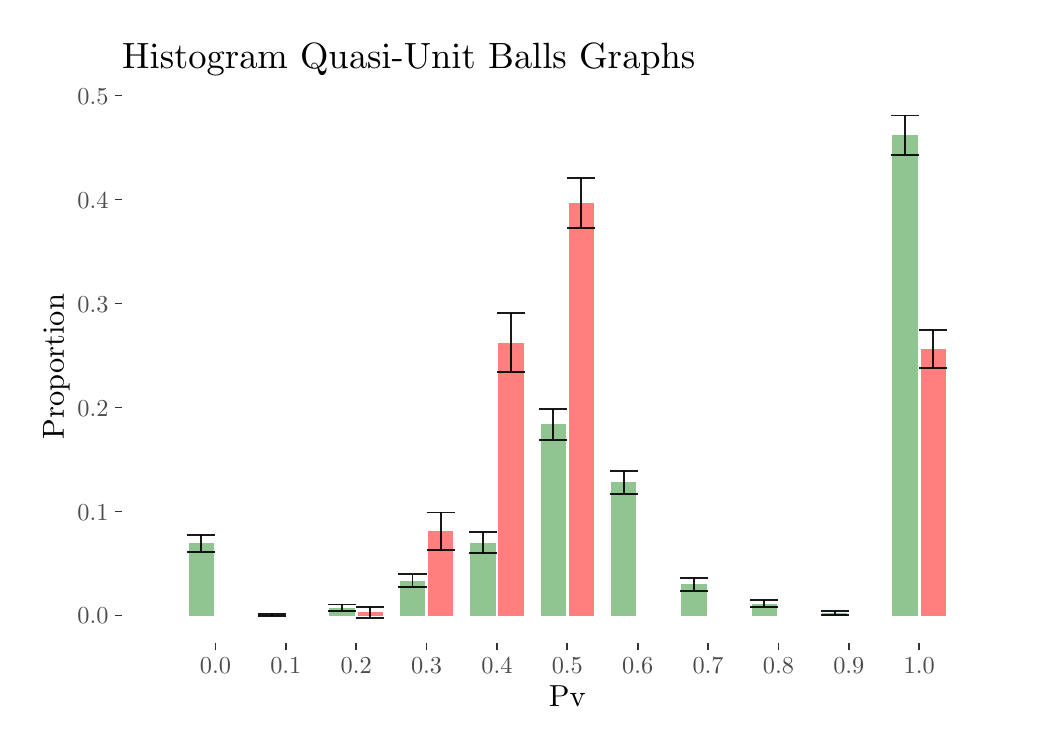
\begin{tikzpicture}[x=1pt,y=1pt]
\definecolor{fillColor}{RGB}{255,255,255}
\path[use as bounding box,fill=fillColor,fill opacity=0.00] (0,0) rectangle (361.35,252.94);
\begin{scope}
\path[clip] (  0.00,  0.00) rectangle (361.35,252.94);
\definecolor{drawColor}{RGB}{255,255,255}
\definecolor{fillColor}{RGB}{255,255,255}

\path[draw=drawColor,line width= 0.6pt,line join=round,line cap=round,fill=fillColor] (  0.00,  0.00) rectangle (361.35,252.94);
\end{scope}
\begin{scope}
\path[clip] ( 34.16, 30.69) rectangle (355.85,230.29);
\definecolor{fillColor}{RGB}{255,255,255}

\path[fill=fillColor] ( 34.16, 30.69) rectangle (355.85,230.29);
\definecolor{fillColor}{RGB}{34,139,34}

\path[fill=fillColor,fill opacity=0.50] ( 58.19, 40.49) rectangle ( 67.34, 66.58);

\path[fill=fillColor,fill opacity=0.50] ( 83.62, 40.49) rectangle ( 92.77, 40.77);

\path[fill=fillColor,fill opacity=0.50] (109.05, 40.49) rectangle (118.20, 43.34);

\path[fill=fillColor,fill opacity=0.50] (134.48, 40.49) rectangle (143.63, 53.15);

\path[fill=fillColor,fill opacity=0.50] (159.91, 40.49) rectangle (169.06, 66.88);

\path[fill=fillColor,fill opacity=0.50] (185.34, 40.49) rectangle (194.49,109.55);

\path[fill=fillColor,fill opacity=0.50] (210.77, 40.49) rectangle (219.92, 88.70);

\path[fill=fillColor,fill opacity=0.50] (236.20, 40.49) rectangle (245.36, 51.75);

\path[fill=fillColor,fill opacity=0.50] (261.63, 40.49) rectangle (270.79, 44.82);

\path[fill=fillColor,fill opacity=0.50] (287.06, 40.49) rectangle (296.22, 41.43);

\path[fill=fillColor,fill opacity=0.50] (312.49, 40.49) rectangle (321.65,214.13);
\definecolor{fillColor}{RGB}{255,0,0}

\path[fill=fillColor,fill opacity=0.50] (119.22, 40.49) rectangle (128.38, 41.76);

\path[fill=fillColor,fill opacity=0.50] (144.65, 40.49) rectangle (153.81, 71.00);

\path[fill=fillColor,fill opacity=0.50] (170.08, 40.49) rectangle (179.24,139.17);

\path[fill=fillColor,fill opacity=0.50] (195.51, 40.49) rectangle (204.67,189.46);

\path[fill=fillColor,fill opacity=0.50] (322.66, 40.49) rectangle (331.82,136.81);
\definecolor{drawColor}{RGB}{0,0,0}

\path[draw=drawColor,draw opacity=0.90,line width= 0.7pt,line join=round] ( 57.68, 69.57) --
	( 67.85, 69.57);

\path[draw=drawColor,draw opacity=0.90,line width= 0.7pt,line join=round] ( 62.77, 69.57) --
	( 62.77, 63.60);

\path[draw=drawColor,draw opacity=0.90,line width= 0.7pt,line join=round] ( 57.68, 63.60) --
	( 67.85, 63.60);

\path[draw=drawColor,draw opacity=0.90,line width= 0.7pt,line join=round] ( 83.11, 41.12) --
	( 93.28, 41.12);

\path[draw=drawColor,draw opacity=0.90,line width= 0.7pt,line join=round] ( 88.20, 41.12) --
	( 88.20, 40.42);

\path[draw=drawColor,draw opacity=0.90,line width= 0.7pt,line join=round] ( 83.11, 40.42) --
	( 93.28, 40.42);

\path[draw=drawColor,draw opacity=0.90,line width= 0.7pt,line join=round] (108.54, 44.51) --
	(118.71, 44.51);

\path[draw=drawColor,draw opacity=0.90,line width= 0.7pt,line join=round] (113.63, 44.51) --
	(113.63, 42.17);

\path[draw=drawColor,draw opacity=0.90,line width= 0.7pt,line join=round] (108.54, 42.17) --
	(118.71, 42.17);

\path[draw=drawColor,draw opacity=0.90,line width= 0.7pt,line join=round] (133.97, 55.42) --
	(144.14, 55.42);

\path[draw=drawColor,draw opacity=0.90,line width= 0.7pt,line join=round] (139.06, 55.42) --
	(139.06, 50.87);

\path[draw=drawColor,draw opacity=0.90,line width= 0.7pt,line join=round] (133.97, 50.87) --
	(144.14, 50.87);

\path[draw=drawColor,draw opacity=0.90,line width= 0.7pt,line join=round] (159.40, 70.74) --
	(169.57, 70.74);

\path[draw=drawColor,draw opacity=0.90,line width= 0.7pt,line join=round] (164.49, 70.74) --
	(164.49, 63.03);

\path[draw=drawColor,draw opacity=0.90,line width= 0.7pt,line join=round] (159.40, 63.03) --
	(169.57, 63.03);

\path[draw=drawColor,draw opacity=0.90,line width= 0.7pt,line join=round] (184.83,115.31) --
	(195.00,115.31);

\path[draw=drawColor,draw opacity=0.90,line width= 0.7pt,line join=round] (189.92,115.31) --
	(189.92,103.78);

\path[draw=drawColor,draw opacity=0.90,line width= 0.7pt,line join=round] (184.83,103.78) --
	(195.00,103.78);

\path[draw=drawColor,draw opacity=0.90,line width= 0.7pt,line join=round] (210.26, 92.86) --
	(220.43, 92.86);

\path[draw=drawColor,draw opacity=0.90,line width= 0.7pt,line join=round] (215.35, 92.86) --
	(215.35, 84.54);

\path[draw=drawColor,draw opacity=0.90,line width= 0.7pt,line join=round] (210.26, 84.54) --
	(220.43, 84.54);

\path[draw=drawColor,draw opacity=0.90,line width= 0.7pt,line join=round] (235.69, 54.11) --
	(245.86, 54.11);

\path[draw=drawColor,draw opacity=0.90,line width= 0.7pt,line join=round] (240.78, 54.11) --
	(240.78, 49.40);

\path[draw=drawColor,draw opacity=0.90,line width= 0.7pt,line join=round] (235.69, 49.40) --
	(245.86, 49.40);

\path[draw=drawColor,draw opacity=0.90,line width= 0.7pt,line join=round] (261.12, 46.08) --
	(271.29, 46.08);

\path[draw=drawColor,draw opacity=0.90,line width= 0.7pt,line join=round] (266.21, 46.08) --
	(266.21, 43.56);

\path[draw=drawColor,draw opacity=0.90,line width= 0.7pt,line join=round] (261.12, 43.56) --
	(271.29, 43.56);

\path[draw=drawColor,draw opacity=0.90,line width= 0.7pt,line join=round] (286.55, 42.04) --
	(296.72, 42.04);

\path[draw=drawColor,draw opacity=0.90,line width= 0.7pt,line join=round] (291.64, 42.04) --
	(291.64, 40.82);

\path[draw=drawColor,draw opacity=0.90,line width= 0.7pt,line join=round] (286.55, 40.82) --
	(296.72, 40.82);

\path[draw=drawColor,draw opacity=0.90,line width= 0.7pt,line join=round] (311.98,221.21) --
	(322.15,221.21);

\path[draw=drawColor,draw opacity=0.90,line width= 0.7pt,line join=round] (317.07,221.21) --
	(317.07,207.05);

\path[draw=drawColor,draw opacity=0.90,line width= 0.7pt,line join=round] (311.98,207.05) --
	(322.15,207.05);

\path[draw=drawColor,draw opacity=0.90,line width= 0.7pt,line join=round] (118.71, 43.76) --
	(128.88, 43.76);

\path[draw=drawColor,draw opacity=0.90,line width= 0.7pt,line join=round] (123.80, 43.76) --
	(123.80, 39.76);

\path[draw=drawColor,draw opacity=0.90,line width= 0.7pt,line join=round] (118.71, 39.76) --
	(128.88, 39.76);

\path[draw=drawColor,draw opacity=0.90,line width= 0.7pt,line join=round] (144.14, 77.75) --
	(154.31, 77.75);

\path[draw=drawColor,draw opacity=0.90,line width= 0.7pt,line join=round] (149.23, 77.75) --
	(149.23, 64.26);

\path[draw=drawColor,draw opacity=0.90,line width= 0.7pt,line join=round] (144.14, 64.26) --
	(154.31, 64.26);

\path[draw=drawColor,draw opacity=0.90,line width= 0.7pt,line join=round] (169.57,149.98) --
	(179.74,149.98);

\path[draw=drawColor,draw opacity=0.90,line width= 0.7pt,line join=round] (174.66,149.98) --
	(174.66,128.36);

\path[draw=drawColor,draw opacity=0.90,line width= 0.7pt,line join=round] (169.57,128.36) --
	(179.74,128.36);

\path[draw=drawColor,draw opacity=0.90,line width= 0.7pt,line join=round] (195.00,198.48) --
	(205.18,198.48);

\path[draw=drawColor,draw opacity=0.90,line width= 0.7pt,line join=round] (200.09,198.48) --
	(200.09,180.43);

\path[draw=drawColor,draw opacity=0.90,line width= 0.7pt,line join=round] (195.00,180.43) --
	(205.18,180.43);

\path[draw=drawColor,draw opacity=0.90,line width= 0.7pt,line join=round] (322.15,143.76) --
	(332.33,143.76);

\path[draw=drawColor,draw opacity=0.90,line width= 0.7pt,line join=round] (327.24,143.76) --
	(327.24,129.86);

\path[draw=drawColor,draw opacity=0.90,line width= 0.7pt,line join=round] (322.15,129.86) --
	(332.33,129.86);
\end{scope}
\begin{scope}
\path[clip] (  0.00,  0.00) rectangle (361.35,252.94);
\definecolor{drawColor}{gray}{0.30}

\node[text=drawColor,anchor=base east,inner sep=0pt, outer sep=0pt, scale=  0.88] at ( 29.21, 37.46) {0.0};

\node[text=drawColor,anchor=base east,inner sep=0pt, outer sep=0pt, scale=  0.88] at ( 29.21, 75.03) {0.1};

\node[text=drawColor,anchor=base east,inner sep=0pt, outer sep=0pt, scale=  0.88] at ( 29.21,112.61) {0.2};

\node[text=drawColor,anchor=base east,inner sep=0pt, outer sep=0pt, scale=  0.88] at ( 29.21,150.19) {0.3};

\node[text=drawColor,anchor=base east,inner sep=0pt, outer sep=0pt, scale=  0.88] at ( 29.21,187.76) {0.4};

\node[text=drawColor,anchor=base east,inner sep=0pt, outer sep=0pt, scale=  0.88] at ( 29.21,225.34) {0.5};
\end{scope}
\begin{scope}
\path[clip] (  0.00,  0.00) rectangle (361.35,252.94);
\definecolor{drawColor}{gray}{0.20}

\path[draw=drawColor,line width= 0.6pt,line join=round] ( 31.41, 40.49) --
	( 34.16, 40.49);

\path[draw=drawColor,line width= 0.6pt,line join=round] ( 31.41, 78.06) --
	( 34.16, 78.06);

\path[draw=drawColor,line width= 0.6pt,line join=round] ( 31.41,115.64) --
	( 34.16,115.64);

\path[draw=drawColor,line width= 0.6pt,line join=round] ( 31.41,153.22) --
	( 34.16,153.22);

\path[draw=drawColor,line width= 0.6pt,line join=round] ( 31.41,190.79) --
	( 34.16,190.79);

\path[draw=drawColor,line width= 0.6pt,line join=round] ( 31.41,228.37) --
	( 34.16,228.37);
\end{scope}
\begin{scope}
\path[clip] (  0.00,  0.00) rectangle (361.35,252.94);
\definecolor{drawColor}{gray}{0.20}

\path[draw=drawColor,line width= 0.6pt,line join=round] ( 67.85, 27.94) --
	( 67.85, 30.69);

\path[draw=drawColor,line width= 0.6pt,line join=round] ( 93.28, 27.94) --
	( 93.28, 30.69);

\path[draw=drawColor,line width= 0.6pt,line join=round] (118.71, 27.94) --
	(118.71, 30.69);

\path[draw=drawColor,line width= 0.6pt,line join=round] (144.14, 27.94) --
	(144.14, 30.69);

\path[draw=drawColor,line width= 0.6pt,line join=round] (169.57, 27.94) --
	(169.57, 30.69);

\path[draw=drawColor,line width= 0.6pt,line join=round] (195.00, 27.94) --
	(195.00, 30.69);

\path[draw=drawColor,line width= 0.6pt,line join=round] (220.43, 27.94) --
	(220.43, 30.69);

\path[draw=drawColor,line width= 0.6pt,line join=round] (245.86, 27.94) --
	(245.86, 30.69);

\path[draw=drawColor,line width= 0.6pt,line join=round] (271.29, 27.94) --
	(271.29, 30.69);

\path[draw=drawColor,line width= 0.6pt,line join=round] (296.72, 27.94) --
	(296.72, 30.69);

\path[draw=drawColor,line width= 0.6pt,line join=round] (322.15, 27.94) --
	(322.15, 30.69);
\end{scope}
\begin{scope}
\path[clip] (  0.00,  0.00) rectangle (361.35,252.94);
\definecolor{drawColor}{gray}{0.30}

\node[text=drawColor,anchor=base,inner sep=0pt, outer sep=0pt, scale=  0.88] at ( 67.85, 19.68) {0.0};

\node[text=drawColor,anchor=base,inner sep=0pt, outer sep=0pt, scale=  0.88] at ( 93.28, 19.68) {0.1};

\node[text=drawColor,anchor=base,inner sep=0pt, outer sep=0pt, scale=  0.88] at (118.71, 19.68) {0.2};

\node[text=drawColor,anchor=base,inner sep=0pt, outer sep=0pt, scale=  0.88] at (144.14, 19.68) {0.3};

\node[text=drawColor,anchor=base,inner sep=0pt, outer sep=0pt, scale=  0.88] at (169.57, 19.68) {0.4};

\node[text=drawColor,anchor=base,inner sep=0pt, outer sep=0pt, scale=  0.88] at (195.00, 19.68) {0.5};

\node[text=drawColor,anchor=base,inner sep=0pt, outer sep=0pt, scale=  0.88] at (220.43, 19.68) {0.6};

\node[text=drawColor,anchor=base,inner sep=0pt, outer sep=0pt, scale=  0.88] at (245.86, 19.68) {0.7};

\node[text=drawColor,anchor=base,inner sep=0pt, outer sep=0pt, scale=  0.88] at (271.29, 19.68) {0.8};

\node[text=drawColor,anchor=base,inner sep=0pt, outer sep=0pt, scale=  0.88] at (296.72, 19.68) {0.9};

\node[text=drawColor,anchor=base,inner sep=0pt, outer sep=0pt, scale=  0.88] at (322.15, 19.68) {1.0};
\end{scope}
\begin{scope}
\path[clip] (  0.00,  0.00) rectangle (361.35,252.94);
\definecolor{drawColor}{RGB}{0,0,0}

\node[text=drawColor,anchor=base,inner sep=0pt, outer sep=0pt, scale=  1.10] at (195.00,  7.64) {Pv};
\end{scope}
\begin{scope}
\path[clip] (  0.00,  0.00) rectangle (361.35,252.94);
\definecolor{drawColor}{RGB}{0,0,0}

\node[text=drawColor,rotate= 90.00,anchor=base,inner sep=0pt, outer sep=0pt, scale=  1.10] at ( 13.08,130.49) {Proportion};
\end{scope}
\begin{scope}
\path[clip] (  0.00,  0.00) rectangle (361.35,252.94);
\definecolor{drawColor}{RGB}{0,0,0}

\node[text=drawColor,anchor=base west,inner sep=0pt, outer sep=0pt, scale=  1.32] at ( 34.16,238.35) {Histogram Quasi-Unit Balls Graphs};
\end{scope}
\end{tikzpicture}
